% Factorisation patterns of X^5-X-1 mod p, 17982 primes p<200000, against the cycle types of S_5 (generated).
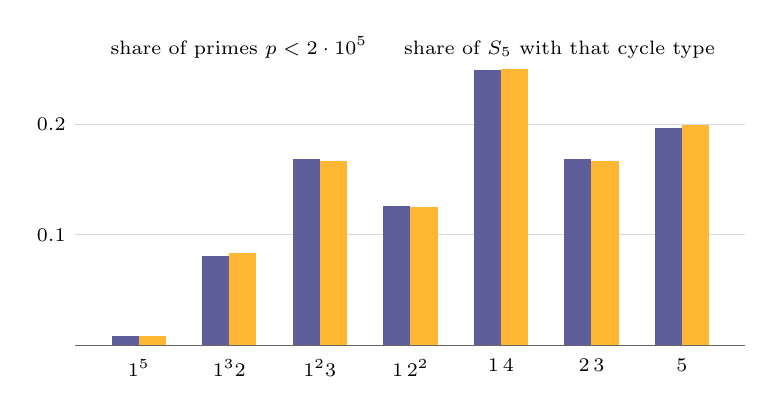
\begin{tikzpicture}[yscale=14,xscale=1.15]
\draw[black!60] (0.3,0)--(7.7,0);
\draw[black!15] (0.3,0.10)--(7.7,0.10); \node[font=\scriptsize,anchor=east] at (0.3,0.10) {$0.1$};
\draw[black!15] (0.3,0.20)--(7.7,0.20); \node[font=\scriptsize,anchor=east] at (0.3,0.20) {$0.2$};
\fill[MidnightBlue!70] (0.70,0) rectangle (1.00,0.0083);
\fill[Orange!80] (1.00,0) rectangle (1.30,0.0083);
\node[font=\scriptsize,anchor=north] at (1,-0.004) {$1^5$};
\fill[MidnightBlue!70] (1.70,0) rectangle (2.00,0.0806);
\fill[Orange!80] (2.00,0) rectangle (2.30,0.0833);
\node[font=\scriptsize,anchor=north] at (2,-0.004) {$1^3 2$};
\fill[MidnightBlue!70] (2.70,0) rectangle (3.00,0.1691);
\fill[Orange!80] (3.00,0) rectangle (3.30,0.1667);
\node[font=\scriptsize,anchor=north] at (3,-0.004) {$1^2 3$};
\fill[MidnightBlue!70] (3.70,0) rectangle (4.00,0.1262);
\fill[Orange!80] (4.00,0) rectangle (4.30,0.1250);
\node[font=\scriptsize,anchor=north] at (4,-0.004) {$1\,2^2$};
\fill[MidnightBlue!70] (4.70,0) rectangle (5.00,0.2495);
\fill[Orange!80] (5.00,0) rectangle (5.30,0.2500);
\node[font=\scriptsize,anchor=north] at (5,-0.004) {$1\,4$};
\fill[MidnightBlue!70] (5.70,0) rectangle (6.00,0.1689);
\fill[Orange!80] (6.00,0) rectangle (6.30,0.1667);
\node[font=\scriptsize,anchor=north] at (6,-0.004) {$2\,3$};
\fill[MidnightBlue!70] (6.70,0) rectangle (7.00,0.1972);
\fill[Orange!80] (7.00,0) rectangle (7.30,0.2000);
\node[font=\scriptsize,anchor=north] at (7,-0.004) {$5$};
\node[font=\scriptsize,anchor=west] at (0.5,0.27) {\textcolor{MidnightBlue!70}{$\blacksquare$} share of primes $p<2\cdot10^5$ \quad \textcolor{Orange!80}{$\blacksquare$} share of $S_5$ with that cycle type};
\end{tikzpicture}
